% !TeX root = ../thesis.tex

\subsection{Introduction}

With the growing technological advances, the quantity of healthcare-related data produced around the world increased exponentially \cite{choi_generating_2017,henry_adoption_2016}.
Consequently, the potential for harvesting this data also increases. The value locked within
this data could help provide better healthcare with new information about diseases,
drugs, and preventive therapies. It can also help create better \acp{his}, meaning an overall better clinical practice \cite{ISI:000502534100049}. But for this to happen, data must reach capable hands at the right time.
But the release of clinical data has several barriers attached and rightly so. The leakage of patient’s privacy can break the confidence of the population in healthcare
professionals and institutions. Patient safety
and privacy should be kept at all costs. However, the current mechanisms for privacy maintenance are very long, bureaucratic, and time-consuming, nationally \cite{comissao_nacional_protecao_de_dados_principios_2015}, and internationally \cite{office_for_civil_rights_guidance_2013}. The current scenario and general methods for privacy safeguards are related to pseudo-anonymisation techniques.
The removal of certain attributes, identifier modification, code grouping, or discretization are some methodologies. But not even these are totally safe \cite{el_emam_systematic_2011}.
Synthetic data appear as an alternative for clinical data sharing, promising great data
utility with minimal privacy concerns. Synthetic data is data that is generated automatically through programmatic processes. This is especially impactful for the case at hand
since synthetic data has no explicit connection with the original data. There are several
mechanisms for data synthesis postulated by \cite{goncalves_generation_2020}, there are
process-driven methods and data-driven methods. Process-driven methods generate
data through pre-determined models inputted into the generator. Data-driven methods
produce new data based on inputted source data. With this, it is possible to create new
patient data that has no relation to reality while providing the same statistical relations
between variables. This provides the basis for quality clinical research on top of this
new data. Even though these techniques are still new and in rapid development, the
results seem interesting \cite{goncalves_generation_2020}, but not without questions and doubts
\cite{stadler_synthetic_2020}.
Creating a thorough survey based on the generation of synthetic data is seldom a simple task when compared to other surveys since synthetic data is present across several domains and has several uses, like software testing, assessing methods, or generating hypotheses. Moreover, synthesis has
the double meaning of summing up information and generating something, easily wielding hundreds of results per query. Finally, trying to filter
algorithms aimed at tabular data is also burdensome, since not always it is easy to discriminate input types. These factors make the survey interesting to focus on the state-of-the-art mechanisms of generating tabular data.

\subsection{Theoretical background}
First introduced in 2014, \acp{gan} \cite{goodfellow_generative_2014} have been under the scope and have been proven very good for generating complex data. Images, text, and video have been successfully generated with very good performances. %cite?
The original architecture is based on two artificial neural networks trained simultaneously in a competitive manner. One of them, the generator, has the objective of generating the most realistic possible data, while the second network – the discriminator, has the opposite aim of aiming to distinguish the realistic data from the synthetic
data the best it can. So, the elegance of this architecture is that each network tries to
make the other perform better every time. The \ac{gan} architecture is shown in \ref{fig:gan-arch}.
% w - \omega
% θ - \theta
% G - generator
% D - discriminator

\begin{figure}
\centering
%\includegraphics[width=\textwidth]{image.png}
\includegraphics[scale=0.75]{figures/image.png}

\caption{\ac{gan} framework} \label{fig:gan-arch}
\end{figure}
The generator is represented by $G_{\theta}$ where the parameter $\theta$ represents the weights of
the neural network. It takes as input, a Gaussian random variable, and outputs $G_{\theta}$(Z).
Distribution of $G_{\theta}$(Z) is denoted by $P_{\theta}$. The goal of the generator is to choose $\theta$ such that the output $G_{\theta}$(Z) has a distribution close to the real data. The discriminator is represented by $D_{\omega}$, parametrized by weights $\omega$. The goal of the discriminator is to assign 1 to the samples from the real distribution $P_{X}$ and 0 to the generated samples ($P_{\theta}$). So, \acp{gan} can be mathematically represented by a minmax game identified by:
\begin{equation}
\min_{G}\max_{D} \; E [log(D_{\omega}(X)) + log(1-D_{\omega}(G_{\theta}(Z))]
\end{equation}
So, G must minimize this equation and D must maximize it, each one tweaking the weights of its network ($\theta$ and $\omega$) to do so. This is the loss function on the initial \ac{gan} architecture. After the classification of D, the G is trained again with the error signal from D through backpropagation. This equation is the log of the probability of D predicting that the real data is genuine and the log probability of D classifying synthetic data as not genuine. The equation is essentially the same as minimising the \ac{jsd} \cite{goodfellow_generative_2014}:
\begin{equation}
\min_{G} JS(P_{x}||P_{\theta})
\end{equation}
Where the JS means the \acl{jsd} between the probability of the real
data and the probability of the generated data. The JS divergence provides a measure
of the distance between two probability distributions. Therefore, the minimization over $\theta$
means, choosing the $P_{\theta}$ that is closest to the target distribution $P_{X}$ in the JS divergence
distance. Despite the significant results provided by \acp{gan} with continuous real values, categorical values still seem to be a problem for this approach \cite{kusner_gans_2016}, since it is not directly applicable for calculating the gradients of latent
categorical variables in order to train these networks through backpropagation. This
happens since the output of the generator, even though can be transformed into a multinomial distribution with a softmax layer, sampling from it is not a differentiable operation, limiting the backpropagation process of the \ac{gan}.

%One of the most famous alternative GAN architectures is the \textit{Wasserstein}  GAN (WGAN)
%\cite{arjovsky_wasserstein_2017} . It improves GAN by using the \textit{Wasserstein} distance instead of the \textit{Jensen-shannon divergence}. It is represented by the
%following minimax game:
%\begin{equation}
%\min_{G}\max_{\omega \; \epsilon \;W} \;\; E[f_{\omega}(X)] - E[f_{\omega}(G_{\theta}(Z))] 
%\end{equation} 
%Where functions $f_{\omega} \;  \omega \; \epsilon \;W$  are all \textit{K-Lipschitz} (with respect to $x$) for some K.
%This was proposed because it helps prevent mode collapse, where the generator maps
%several inputs to the same output. An example of this is a generator that starts creating
%several images with the same patterns or colours. The fact that this loss function can be
%very customisable in distinct GAN implementation, applying different functions can
%lead to different outcomes and architectures.

%\iffalse
%\subsubsubsection{Differential privacy}
%The privacy model most used in generative models is differential privacy \cite{dwork_differential_2006}. It is a mathematical model for measuring privacy loss. The basis of it is a mechanism that adds noise to a dataset through randomisation. Applying differential privacy is a method for guaranteeing that adding or removing any record from the original data does not influence the generation output. The formal definition, as stated in \cite{dwork_differential_2006} is:
%\begin{equation}
%Pr[M(x)\; \epsilon \; S] \leq e^\varepsilon Pr[M(y)\; \epsilon \; S] + \delta
%\end{equation} 
%Where M is a randomised mechanism, $\varepsilon$ is the privacy budget (balance between privacy and utility). The $x$ and $y$ represent adjacent datasets that differ on only one record. So, we say that M gives $\varepsilon$-differential privacy if the probability of seeing an event S in the $x$ dataset is at most equal to $e^\varepsilon$ multiplied by the probability that we see S when the dataset is $y$. Variable $\delta$ is the probability of an uncontrolled breach. With this, a smaller $\varepsilon$ will yield better privacy but a less accurate response, so it can be used to tweak the utility and privacy of the dataset.
%\fi

\subsection{Methods}
This search was made between December 2020 and January 2021. It was made on “Web of Science”, IEEE, PubMed, Arxiv and finally GitHub. The terms searched were related to \acp{gan}, synthetic data generation, electronic health records, patient data, or tabular data. Applications of \acp{gan} to non-tabular data were filtered, like image, sound, video, or graphs. Time series and text data were also removed since the methodology for synthesizing this type of data has specific functions related to the nature of the data. The filter for date was after 2014 since \acp{gan} were introduced at that time. The queries used were similar to the one below, adapted for the search mechanics for each website.


\begin{scriptsize}

{\fontfamily{courier}\selectfont
("generation" OR "creation" OR "synthesis" OR "synthesizing" OR "generating" OR "creating") AND ("synthetic data" OR "synthetic patient" OR "synthetic electronic health record" OR "synthetic EHR" OR "realistic patient data" OR "realistic health record" OR ("synthetic" AND "privacy" AND "utility"))  AND ("GAN" OR "Generative Adversarial Network")}
\end{scriptsize}
%\begin{verbnobox}[\scriptsize]
%("generation" OR "creation" OR "synthesis" OR "synthesizing" OR
%"generating" OR "creating") AND ("synthetic data" OR
%"synthetic patient" OR "synthetic electronic health record" 
%OR "synthetic EHR" OR "realistic patient data" OR "realistic 
%health record" OR ("synthetic" AND "privacy"  AND "utility")) 
%AND ("GAN" OR "Generative Adversarial Network")
%\end{verbnobox}

From the total articles found (1165) with all the queries, 100 articles were chosen for full text and in the end, 22 papers with \ac{gan} implementations that were tested on tabular data were selected. 
%These implementations were studied and evaluated in terms of privacy concerns and utility performance and compared when possible. 
%For selecting the articles and helping with paper selection, RAYYAN QCRI online \cite{rayyan:14:cochrane} was used along with Mendeley Reference Manager for paper management.


\subsection{Results}
The selected papers ranged from 2017 to 2020. Being that 2 are from 2017, 4 from 2018, 8 from 2019 and 8 from 2020. All authors showed original \ac{gan} implementations, apart from 2 papers. Beaulieu-Jones et al. \cite{beaulieu-jones_privacy-preserving_2019} used a
\ac{gan} architecture that was originally published with usage on image datasets \cite{odena_conditional_2017}. Additionally, Vega-Marquez et al.  \cite{ISI:000490706700022} used an already known implementation of conditional \acp{gan} \cite{mirza_conditional_2014}. We classified papers regarding 3 metrics: utility, privacy and clinical. For utility, we looked for  methods for measuring the generated data's quality. As for privacy, we aimed for some mechanism for measuring the privacy loss of the new data. Concerning clinical metrics, any kind of evaluation from healthcare professionals was considered. This can be seen in table \ref{tab:review_gans}.


\begin{table}[btph]
\caption{Summary of the articles selected.}\label{tab:review_gans}
\centering
\begin{tabular}{l|llclc}
%\begin{tabular}{l|llclc}

\toprule
 ID & year  & Acronym & Article & Metric & Code \\

% & \multicolumn{1}{|c}{Year \hspace{2 mm}}  & \multicolumn{1}{|c|}{Acronym} & \multicolumn{1}{c}{\hspace{2 mm} Article \hspace{1 mm}} & \multicolumn{1}{|c|}{Metric} & \multicolumn{1}{c|}{\hspace{2 mm}Code \hspace{2 mm}}  \\

\midrule
1 & 2017 & medGAN  &\cite{choi_generating_2017}          & Utility, Privacy, Clinical \hspace{1 mm} &  \cite{medGANurl}  \\

2 & 2017 & POSTER & \cite{ISI:000440307700174} & Utility, Privacy  &   \cite{POSTERurl}\\

3 & 2018 & table-GAN & \cite{park_data_2018} & Utility, Privacy         &   \cite{table-GAN-url} \\

4 & 2018 & dp-GAN & \cite{xie_differentially_2018}& Utility, Privacy &   \cite{dp-GAN-url}  \\

5 & 2018 & mc-medGAN & \begin{tabular}[c]{@{}l@{}}\cite{camino_generating_2018}\end{tabular}    & Utility &   \cite{mcmedgan-url}\\

6 & 2018 & TGAN &  \cite{xu_synthesizing_2018}& Utility &  \cite{tgan-url}\\

7 & 2019 & PATE-GAN & \begin{tabular}[c]{@{}l@{}}\cite{jordon_pate-gan_2019}\end{tabular}    & Utility, Privacy   & --\\

8 & 2019 & SPRINT-GAN & \cite{beaulieu-jones_privacy-preserving_2019}           & Utility, Privacy, Clinical &  \cite{sprint-GAN-url} \\

9 & 2019 & GAN-based &     \cite{ISI:000524576200016} & Utility, Privacy & --\\

10 & 2019 & CTGAN &  \cite{xu_modeling_2019} & Utility & \cite{CTGAN-url}\\

11 & 2019 & WGAN-DP & \begin{tabular}[c]{@{}l@{}}\cite{brenninkmeijer_generation_2019}\end{tabular} & Utility, Privacy    & \cite{WGAN-DP-url} \\

12 & 2019 & PPGAN &  \cite{liu_ppgan_2019} & Utility, Privacy &  \cite{ppgan-url}\\

13 & 2019 & medBGAN &   \cite{ISI:000502534100049} & Utility & --\\

14 & 2019 & medWGAN& \cite{medwgan}& Utility &  \cite{medWGAN-url}  \\

15 & 2020 & ADS-GAN& \begin{tabular}[c]{@{}l@{}}\cite{ISI:000557358500024}\end{tabular} & Utility, Privacy& --\\

16 & 2020 & corGAN & \cite{2001.09346}& Utility, Privacy &  \cite{corGAN-url}\\
17 & 2020 & CGAN &  \cite{ISI:000490706700022}& Utility& --\\

18 & 2020 & DPAutoGAN&  \cite{tantipongpipat2020differentially}& Utility, Privacy & \cite{DPAutoGAN-url}\\

19 & 2020 & GAN Boosting& \cite{2007.11934} & Utility, Privacy &  \cite{postganurl}\\

20 & 2020 & RDP-CGAN&  \cite{rdp-gan}& Utility, Privacy &  \cite{rdp-cgan-url}\\

21 & 2020 & WCGAN-GP&  \cite{WCGAN-GP}& Utility, Privacy & --\\
22 & 2020 & SMOOTH-GAN &  \cite{smooth-gan} & Utility & \cite{smooth-gan-url}\\
\hline
\end{tabular}
\end{table}


The metrics the authors used are exhibited in table \ref{tab:results_review}. 



\begin{landscape}
\renewcommand{\arraystretch}{1.02} %add more space between cells (1.2 is a factor)
\begin{table}[htbp]
\caption{Metrics utilised for evaluation} \label{tab:results_review} 

\begin{tabular}{p{26mm} p{84mm} p{60mm}}
\hline
Acronym & Utility & Privacy \\
\hline
medGAN	& \begin{enumerate*}
    \item Bern.
    \item Pred F1
\end{enumerate*} & \begin{enumerate*}
\item Attrib. disc. \item Memb. inf. \item KNN	\end{enumerate*}  \\

%\arrayrulecolor{mygrey}\hline

POSTER &	\begin{enumerate*}
\item Pred Acc.
\item Corre. Mat. \item BD
\end{enumerate*} & DP\\
table-GAN &	\begin{enumerate*}
\item Cumul. Dist.
\item Pred F1$\vert$MRE
 \end{enumerate*} &	\begin{enumerate*} \item Eucl.
\item Member. inf.   \end{enumerate*}  \\

dp-GAN &	\begin{enumerate*} \item Pred AUC \item Bern. \end{enumerate*} &	DP	 \\

mc-medGAN & 	\begin{enumerate*} \item Pred F1$\vert$AUC \item Bern. \item ME F1$\vert$Acc\end{enumerate*} & -- 	\\

TGAN &	\begin{enumerate*} \item KNN \item NMI \item Pred F1 \end{enumerate*} & --\\

PATE-GAN & \begin{enumerate*} \item  Pred AUC$\vert$AUPRC \end{enumerate*}	& DP \\
SPRINT-GAN & \begin{enumerate*}	\item Pred AUC \item Corre. Mat. \end{enumerate*} &	DP \\

GAN-based &	  \begin{enumerate*} \item Pred Acc. \item Corre. Mat. \end{enumerate*} & \begin{enumerate*} \item Hit. Rate \item R. Linkage  \item Eucl. \end{enumerate*} \\

CTGAN &	\begin{enumerate*} \item Pred F1$\vert$R2$\vert$Acc. \end{enumerate*} &  --\\

WGAN-DP &	\begin{enumerate*} \item Corre. Mat.
 \item PCA \item  Pearson RMSE\newline\item Pred F1$\vert$RMSE$\vert$1-MAPE(F1)  \end{enumerate*}  & \begin{enumerate*} \item Eucl. \item Dupl. \item DP \end{enumerate*}	\\

PPGAN &	\begin{enumerate*} \item GS \end{enumerate*}	& DP \\

medBGAN	& \begin{enumerate*}  \item Assoc. Rul.
 \item  CCS Pred F1
\item KS
 \end{enumerate*}	& -- \\

medWGAN	& \begin{enumerate*} \item Assoc. Rul.\item  CCS Pred F1 \item KS \end{enumerate*} & -- \\

ADS-GAN &  \begin{enumerate*} \item $\chi^{2}$ \item JSD \item WD
\item t-test \item Pred AUROC\newline
\item Corre. Mat. \end{enumerate*}	& DP \\

CorGAN &	\begin{enumerate*} \item Pred F1 \item Bern. \end{enumerate*}
 &	Member. Inf. \\

CGAN &	\begin{enumerate*} \item Pearson
\item Spearman \item Pred F1$\vert$AUC$\vert$Acc \end{enumerate*}  &	-- \\

DPAutoGAN & \begin{enumerate*} \item Pred AUROC$\vert$R2  \item Bern. \end{enumerate*}	
 &	DP \\
GAN Boosting & \begin{enumerate*} \item pRMSE \item Pred AUROC$\vert$AUPRC$\vert$Acc. \end{enumerate*}	
	& DP \\
RDP-CGAN & \begin{enumerate*} \item Pred F1$\vert$AUROC$\vert$AUPRC \item MMD  \end{enumerate*}	
	& DP \\
WCGAN-GP & \begin{enumerate*} \item Corre. Mat.
 \item Pred F1  \end{enumerate*} & \begin{enumerate*} \item Dupl.
\item Eucl. \end{enumerate*} \\
SMOOTH-GAN & \begin{enumerate*} \item DW MAE \item Pearson  \item Pred AUROC$\vert$AUPRC \end{enumerate*}	
	& -- \\
\hline

\end{tabular}
\end{table}
\end{landscape}


Regarding privacy, 15 papers assessed it or included some kind of mechanism to improve data protection. The most common was including Differential Privacy (DP) in the generation process. Other mechanisms for measuring privacy loss were Membership Inference (Member. Inf.), Attributes Disclosure (Attrib. Disc.), Euclidean distance (Eucl.), record-linkage (R. Linkage) and Nearest Neighbours (KNN).
As for utility, all papers assessed it. There were 3 major areas of utility assessment: Dimension-wise (DW) probability, cross-testing, and distance metrics. The most basic one was dimension-wise probability, which is important for making sanity checks for the generated data, comparing the distributions of each column between real and synthetic. In this category, we can find Bernoulli (Bern.), cumulative distributions (Cumul. Dist.), Pearson correlation (Pearson) and Spearman correlation (Spearman), correlation coefficients (CCS), chi-squared test ($\chi^{2}$),  \ac{ks} or Correlation Matrices (Corre. Mat.).
Cross-testing was about training machine-learning algorithms with both datasets in order to compare the results. The key factor is generating a synthetic dataset based on the training set and then training models on the original training set and the generated dataset. Then the models are compared regarding their predictive capability on the (real) test set. This was a way of assessing if the generator models were capturing inter-variable relationships. The authors applied different metrics from AUC, F1, \ac{auprc}, Accuracy (Acc.) to \ac{mre}. Finally, there was also the application of distance metrics, for measuring the difference between column distribution in both datasets. \acl{jsd}, Wasserstein Distance (WD), Bhattacharyya Distance (BD) or Generate Scores (GS) that was a metric implemented by the authors of \cite{liu_ppgan_2019} that creates a metric based on the sum of the mean of \textit{kullblack-leibler}  distance of all columns. Other less used methods were \ac{pca}, propensity score mean squared error ratio (pMSE). NMI (Normalised Mutual Information), which is the ability to capture correlations between columns by computing the pairwise mutual information and MMD (Maximum Mean Discrepancy), which is similar to distance metrics were also used. Regarding datasets utilized, the most used was MIMIC-III \cite{mimiciii} (9 times). The papers used 27 different datasets, being 16 healthcare-related and 11 non-healthcare related. 
Finally, regarding clinical evaluation, only two papers assessed it, as it is possible to see in table \ref{tab:review_gans}. Both had a group of clinicians assessing a sample of both real and synthetic information and evaluating from 0 to 10, where 10 is the most realistic.
One major point preventing a larger comparison is that despite some papers using the same dataset and same methodologies, the presented values are different, making it difficult for a clear comparison of results. One example is a dimension-wise prediction with F1 score for MIMIC-III. CorGAN presents the mean difference between the two classifications (real on real and synthetic on synthetic), while medBGAN presents the correlation coefficients of the two, and medGAN only presents the visual comparisons. Regarding code availability, 16 papers had the code publicly available in some form. As of January 2021, papers pointed in table \ref{tab:review_gans} have public code.

%\begin{figure}[h]
%\centering
%\includegraphics[scale=0.50]{Paper_plot.png}
%\includegraphics[scale=0.54]{Rplot01.jpeg}

%\caption{Datasets used for measuring Utility and Privacy.} \label{fig2}
%\end{figure}



\subsection{Implications for future research}
From the work done in this paper, it is clear that synthetic data generation is a growing field. The increasing number of papers through the years as the growing quality in the mechanisms of generating data and assessing its quality is clear proof. 
It also became apparent that privacy and utility in synthetic data represent a delicate balance. The very same definition of differential privacy represents it. The compromise between privacy and utility is real and should be taken into account when creating privacy-demanding datasets.
Creating statistically good tabular datasets is already possible, but that task becomes increasingly difficult if privacy concerns are added. 
However, privacy is also a complex subject, and the context of the setting is important for privacy assessment, which explains the different approaches for evaluating privacy protection of synthetic data.
From this review, we believe that a proper evaluation of synthetic data generators in the healthcare setting with privacy concerns should at least include utility and privacy evaluations. For utility, we believe that evaluating column-wise is a nice first check but insufficient alone.
For table-wise, since there is no fundamental metric for assessing the inter-column correlations between mixed-type variables, cross-testing is the best next thing. Distance metrics are nice to have and seem to have the potential for creating a table-wise metric \cite{metrics}, so presenting them is important. Second, for privacy evaluation, we believe that Differential Privacy in itself is not a guarantee of protection for real patients. More research and depth should be employed when presenting results for such generators; record-linkage and attribute disclosure can provide extra guarantees.
Thirdly, a clinical evaluation should be done as well to understand if the synthetic patients are a reality in the clinical setting. Since the correlations could be correct but clinically (or biologically) they might not make sense. Finally, in the scope of this paper, only \acp{gan} were assessed, but there are more mechanisms for generating data, and could be interesting to assess how all of them perform on the same datasets. There are other methods for handling the mixed data types that regularly appear in clinical settings, like \acp{vae} Gaussian Mixtures, \ac{bn}, and imputation mechanisms, making them excellent candidates for this assessment.



\subsection{Conclusion}
In this paper, we had the opportunity to survey the current framework for generating tabular data using \acp{gan} and which ones were already tested in the healthcare setting. We summarised the utility and privacy metrics employed, and the datasets used to measure them. We analysed the code availability and made suggestions for further work on cataloging, comparing, and assessing synthetic health data generators. A survey with a global benchmark of methodologies, despite being arduous, could yield great results for the community and take the aim of this paper further.